\documentclass[Project Report]{article}
\usepackage{graphicx}
\usepackage{fancyhdr}
\usepackage{url}
\usepackage[margin=1in]{geometry}

\pagestyle{fancy}
\lhead{COMP3005 Final Project Report}
\rhead{Ryan Ayotte SN: 101073548}

\begin{document}

\section{Conceptual Design}
{\centering 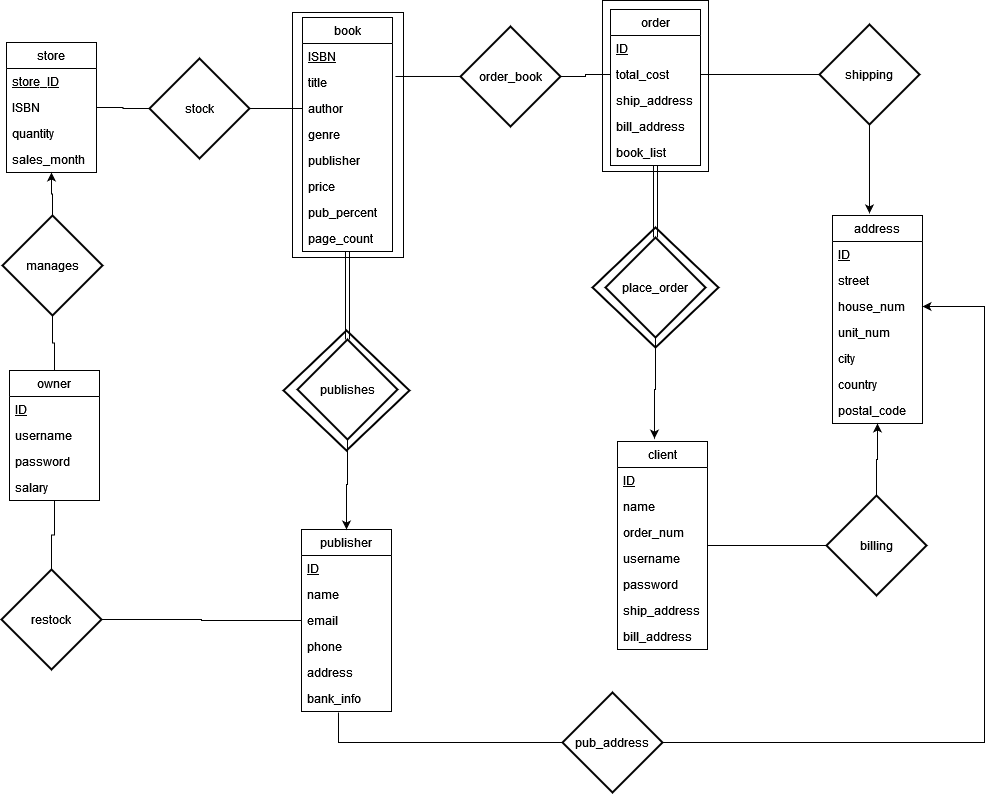
\includegraphics[width=\textwidth]{ER_Diagram.png}}
\begin{itemize}
    \item store: A store is managed by an owner and keeps track of the current stock of each book as well as the sales made for each month
    \item owner: An owner can manage the inventory of the store as well as purchase more from the publishers should stock be running low
    \item book: A book has its stock managed through the store and is published by publishers who also get a percetage of the book's sale. The assumption for a book to exist is that it is first published and provided by the publisher. Books can also be added to orders by the client to be purchased
    \item publisher: A publisher publishes books and provides them to the store owner for their store. They peovide their banking information to receive their part of their book sale, and they have an address they can be reached at
    \item order: An order can be made by a client to buy books from the store and have them sent to the provided shipping address. The assumption for an order to exist is that a client must already exist who have placed the order.
    \item client: A client, who is registered with the store, can place an order of books to be sent to a provided shipping address, paied via their billing address. Assumption is that the addresses were added at time of registration.
    \item report: A report of the sale for the month. It keeps track of the orders made 
\end{itemize}

\section{Reduction to Relation Schemas}
\begin{itemize}
    \item store: (\underline{store\_id})
    \item owner: (\underline{ID}, username, password, salary)
    \item book: (\underline{ISBN}, title, author, genre, publisher, price, pub\_percent, page\_count)
    \item publisher: (\underline{ID}, name, email, phone, address, bank\_info)
    \item order: (\underline{ID}, total\_cost, ship\_address, bill\_address, book\_list, client\_id)
    \item client: (\underline{ID}, name, username, password, ship\_address, bill\_address)
    \item report: (\underline{report\_id}, store\_id, report\_month, report\_sales)
    \item stock: (\underline{ISBN}, quantity)
    \item manages: (\underline{owner\_id}, \underline{store\_id})
    \item publishes: (\underline{ISBN}, \underline{pub\_id})
    \item order\_book: (\underline{ISBN}, \underline{order\_id})
    \item place\_order: (\underline{client\_id}, \underline{order\_id})
    \item generate: (\underline{store\_id}, \underline{report\_id})
    \item logs: (\underline{report\_id}, \underline{order\_id})
\end{itemize}

\section{Normalization of Relation Schemas}

\subsection{Relationship sets}

\subsubsection{stock}
ISBN is the superkey\\
$ISBN \rightarrow quantity$

\subsubsection{manages}
owner\_id and store\_id are superkeys\\\\
Since both attributes are part of the superkey, and they are the only values, then all rows are unique and therefore the relation is in normal form

\subsubsection{publishes}
ISBN and pub\_id are the superkeys\\\\
Since both attributes are part of the superkey, and they are the only values, then all rows are unique and therefore the relation is in normal form

\subsubsection{order\_book}
ISBN and order\_id are the superkeys\\\\
Since both attributes are part of the superkey, and they are the only values, then all rows are unique and therefore the relation is in normal form

\subsubsection{place\_order}
client\_id and order\_id are the superkeys\\\\
Since both attributes are part of the superkey, and they are the only values, then all rows are unique and therefore the relation is in normal form

\subsubsection{generate}
report\_id and store\_id are the superkeys\\\\
Since both attributes are part of the superkey, and they are the only values, then all rows are unique and therefore the relation is in normal form

\subsubsection{logs}
report\_id and order\_id are the superkeys\\\\
Since both attributes are part of the superkey, and they are the only values, then all rows are unique and therefore the relation is in normal form

\newpage
\section{Database Schema Design}
{\centering 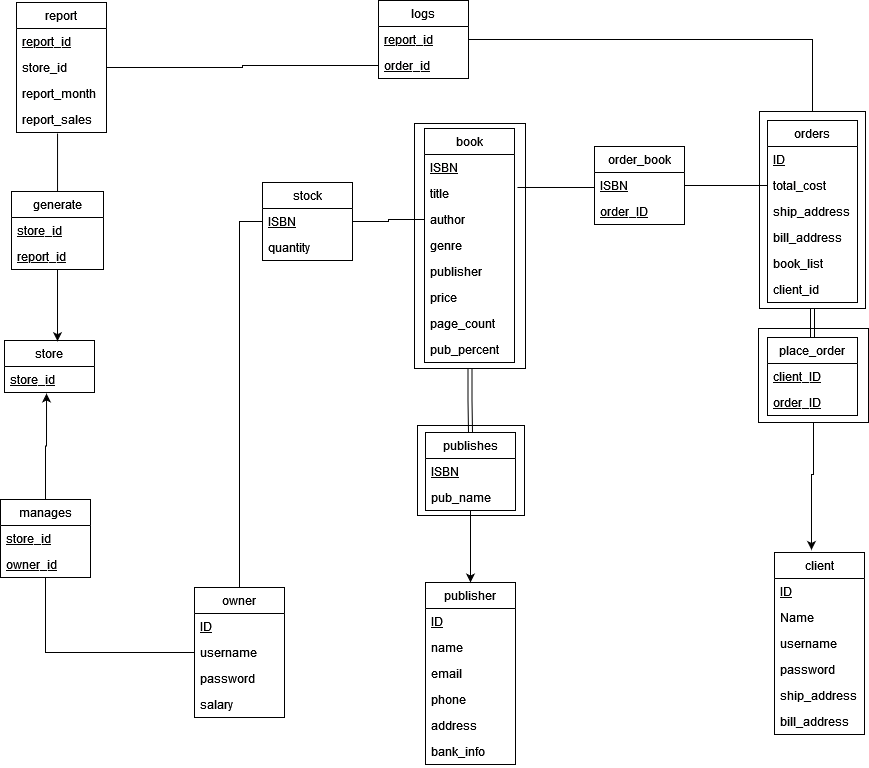
\includegraphics[width=\textwidth]{Schema_Diagram.png}}

\section{Implementation}
Mostly fully complete. Only things missing are the automatic trigger for restocking books (manual option for owners currently), as well as generating sales reports (tables and inserts are there but functionality is not).\\\\\\\\\\\\\\\\\\\\

Login and main menu for client and owners. They must be registered users in order to be authorized\\
{\centering 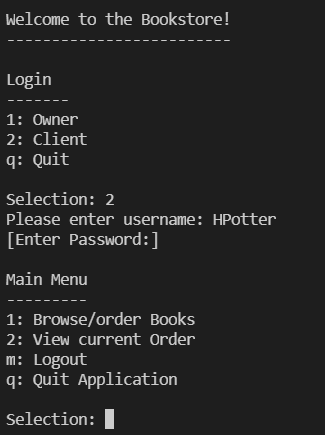
\includegraphics[width=\textwidth]{../Screenshots/Client_login_main_menu.png}}

{\centering 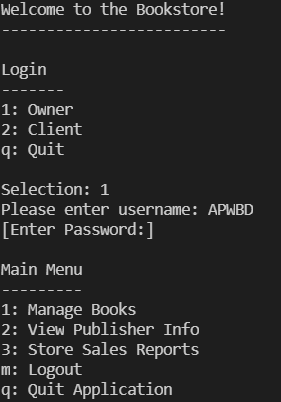
\includegraphics[width=\textwidth]{../Screenshots/Owner_login_main_menu.PNG}}

Client Catalog menu. User can browse for books by auther, genre, or publisher as well as details for a specfic book. They can add books to their order, place their order, and track their orders\\
{\centering 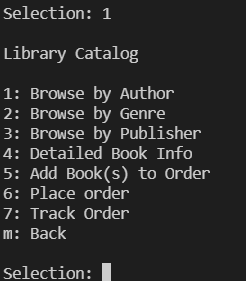
\includegraphics[width=\textwidth]{../Screenshots/Client_Catalog_menu.PNG}}\\\\\\\\\\\\\\\

Client order tracking menu\\
{\centering 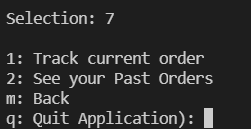
\includegraphics[width=\textwidth]{../Screenshots/Client_order_tracker_menu.PNG}}\\\\\\\\

Client view current order if there is a an order\\
{\centering 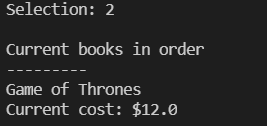
\includegraphics[width=\textwidth]{../Screenshots/Client_view_current_order.PNG}}\\\\\\\\\\\\\\\\\\\

Owner management menu. Owner can restock books, add new books, remove books, and add new publishers\\
{\centering 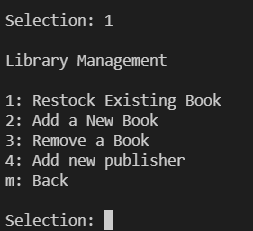
\includegraphics[width=\textwidth]{../Screenshots/Owner_management_menu.PNG}}\\\\\\\\\\\\\\\\\\\\\\\\\\\\\\\\

Owner publisher details screen\\
{\centering 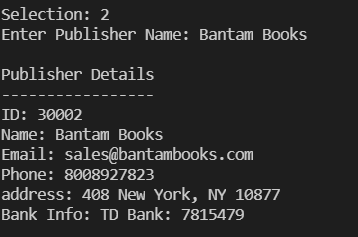
\includegraphics[width=\textwidth]{../Screenshots/Owner_pub_details.PNG}}

\section{Bonus Features}
No bonus features in project

\section{GitHub Repository}
\url{https://github.com/rayotte/COMP_3005_Project}

\section{Appendix I (Availability)}
Exempted from demonstrations based on prior conversation with Professor Roby due to scheduling conflicts

\end{document}